\documentclass{article}
\usepackage[utf8]{inputenc}
\usepackage{mhchem} % símbolos químicos
\usepackage{tabularx}

\usepackage{array} % gestión de tablas
\usepackage{xcolor}
\usepackage{tcolorbox}
\usepackage{graphicx}
\graphicspath{ {imagenes/} }

\tcbset{boxrule=0pt, colback=green!20, arc=0pt, left=0pt, right=0pt}



\title{La nutrición y la digestión}

\begin{document}

	\maketitle
	
	\section{Los nutrientes y los alimentos}
	
		\subsection{Los nutrientes y la nutrición en los animales}
	
			Los \textbf{nutrientes} son las sustancias que proporcionan la energía y la materia que necesita el organismo, como por ejemplo, la glucosa o los aminóacidos. \par
			Se denomina \textbf{nutrición animal} al conjunto de \textbf{reacciones químicas} que permiten a los animales obtener y utilizar los nutrientes presentes en los alimentos. La nutrición incluye los procesos de \textbf{alimentación}, \textbf{digestión} y \textbf{respiración celular}.
	
		\subsection{Tipos de nutrientes}
	
			\begin{itemize}
				\item \textbf{Glúcidos}. Su función principal es aportar energía de uso rápido (aproximadamente 4 kcal/g).Los más sencillos se denominan \textbf{azúcares}.
				\item \textbf{Lípidos}. También denominados \textbf{grasas}. Su función principal es la de ser reserva energética (aproximadamente 9 kcal/g), almacenadas en el tejido adiposo. 
				\item \textbf{Proteínas}. Son las principales moléculas estructurales del cuerpo, proporcionando la materia para el crecimiento y la renovación de los tejidos. Además proporcionan energía, en cantidades similares a los carbohidratos.
				\item \textbf{Agua}. Es la biomoléculas más abundante del cuerpo. No proporciona energía, pero es fundamental para el correcto funcionamiento del cuerpo. 
				\item \textbf{Vitaminas}. Aunque no proporcionan energía son necesarias en pequeñas cantidades. Deben ser ingeridas, ya que el cuerpo es incapaz de sintetizarlas.
				\item \textbf{Minerales}. Realizan muchas y variadas funciones. Por ejemplo, el fostato cálcico y el carbonato cálcico forman parte de los huesos, el ion ferroso (\ce{Fe^2+}) forma parte de la hemoglobina y el ion sodio (\ce{Na^+}) es imprescindible para la transmisión del impulso nervioso.
			\end{itemize}
			
			\par Los glúcidos, los lípidos y las proteínas se denominan \textbf{macronutrientes}, mientras que las vitaminas y las sales minerales son \textbf{micronutrientes}.
			
		\subsection{Tipos de alimentos}
		 
			\begin{center}
			\resizebox{\textwidth}{!}{%
				\begin{tabular}{ | m{3cm} | m{3cm} | m{4cm} | m{4cm} | }
					\hline
					Grupos de alimentos & Ejemplos & Tipo de nutrientes estructurales y micronutrientes & Tipo de nutrientes energéticos \\
					\hline
					Leche y derivados & Leche, yogures y quesos & Proteínas, calcio y vitaminas A, B y D & Lípidos \\
					\hline	
					Carnes, pescados y huevos & Ternera, pollo, merluza, huevos... & Proteínas, hierro y vitamina B2 & Lípidos \\
					\hline 
					Féculas & Patatas, arroz, pan y pasta & Proteínas vegetales, vitamina B1 e hierro & Glúcidos \\
					\hline
					Frutas, verduras y hortalizas & Acelgas, lechuga, pera, uva... & Celulosa, hierro y calcio. En las no hervidas, además, vitaminas A y C & Glúcidos \\
					\hline
					Aceites y grasas & Aceite de oliva, mantequilla, manteca de cerdo... & Vitaminas A y D. En el aceite de oliva y de girasol, además vitamina E & Lípidos \\
					\hline
					Azúcares & Azúcar y caramelos & Ninguno & Glúcidos \\
					\hline
					Bebidas & Agua, zumos, refrescos, vino... & Vitaminas, en los zumos & Glúcidos \\
					\hline
				\end{tabular}
				}
			\end{center}
		
			
	\section{La dieta}
	
		Se llama \textbf{dieta} el tipo, la cantidad y la proporción de alimentos que ingerimos durante un tiempo determinado. \par
		La dieta debe satisfacer las \textbf{necesidades metabólicas} de la persona.
	
		\begin{table}[htp]
			\caption{Recomendaciones nutricionales}
			\begin{center}
				\resizebox{\textwidth}{!}{
				\begin{tabular}{|c|c|c|}
			 		\hline
			 		\textbf{Principios inmediatos} & \textbf{Cantidad máxima diaria}  & \textbf{Advertencias} \\
			 		\hline
			 		\textbf{Glúcidos} & 50-55\% & Los azúcares no pueden superar el 10\% \\
			 		\hline
			 		\textbf{Lípidos} & 30-35\% & Las grasas saturadas no pueden superar el 7\% \\
			 		\hline
			 		\textbf{Proteínas} & 10-15\% & Como mínimo 0,8 g por kilo y día\\
			 		\hline
				\end{tabular}
				}
			\end{center}
			\label{Recomendaciones}
		\end{table}%
	
		Además se recomienda una ingesta mínima fibra vegetal para el buen funcionamiento del tracto intestinal.
		
		\subsection{Hábitos de vida saludables}
	
			\begin{itemize}
				\item Ingerir todo tipo de alimentos.
				\item Consumir diariamente frutas, verduras y hortalizas.
				\item Si se toman grasas, que sean del tipo insaturadas.
				\item Beber entre 1,5 y 2 L de agua al día.
				\item Evitar los alimentos ultraprocesados
				\item Llevar una vida activa, lo que incluyen ejercicio regular y moderado.
				\item Dormir lo necesario.
			\end{itemize}
			
		\subsection{Enfermedades relacionadas con la alimentación}
		
			\subsubsection*{Intoxicaciones e infecciones intestinales}
			
				Provocan fuertes dolores de vientre, vómitos y diarrea.
				
			\subsubsection*{Obesidad}
				Suele deberse a una alimentación en la que abundan los alimentos muy calóricos, junto con una vida con poca actividad física.\par La obesidad supone que el corazón, los pulmones y los riñones, entre otros, deben esforzarse más. 
				  
			\subsubsection*{Transtornos de la conducta alimentaria (TCA)}
			
				\begin{itemize}
					\item \textbf{Anorexia nerviosa}. Se caracteriza por el rechazo a la comida debido al miedo a engordar. Asimismo existe una percepción alterada del propio cuerpo (\textbf{dismorfia corporal}), por lo que la persona se ve a sí misma como obesa, aún en el caso de que esté extremadamente delgada.
					\item \textbf{Bulimia nerviosa}. Se caracteriza por episodios de ingesta excesiva y compulsiva de alimentos, seguidos de una sensación de culpabilidad, que a veces lleva a la provocación del vómito, uso de laxantes, hacer ejercicio intenso...
				\end{itemize}
		
	\section{La nutrición}
	
	\begin{tcolorbox}
		La \textbf{nutrición} es el conjunto de procesos mediante los cuales se transforman y se asimilan los alimentos y se obtienen de ellos la materia y la energía necesaria para el funcionamiento y el crecimiento del organismo.

	\end{tcolorbox}
	
	La nutrición incluye los procesos de \textbf{digestion}, \textbf{respiración}, \textbf{circulación} y \textbf{excreción}.
	
	\section{El aparato digestivo}
		
		El \textbf{aparato digestivo} se encarga de ingerir los alimentos y digerirlos mediante un proceso denominado \textbf{digestión}, hasta que se convierten en moléculas pequeñas capaces de penetrar en las células.
		\par En el \textbf{tubo digestivo} se pueden distinguir seis regiones: cavidad bucal, faringe, esófago, estómago, intestino delgado e intestino grueso.
		\par Al interior del tubo digestivo van a parar las secreciones de las \textbf{glándulas digestivas}, que pueden ser de dos tipos.
		
		\begin{itemize}
			\item \textbf{Glándulas de las paredes del tubo digestivo}. Glándulas del estómago y glándulas intestinales.
			\item \textbf{Glándulas anejas}. Están fuera del tubo digestivo. Por ejemplo, \textbf{glándulas salivales}, \textbf{hígado} y \textbf{páncreas}
		\end{itemize}
		\par Las secreciones de estas glándulas son los llamados \textbf{jugos gástricos}.
		
		\subsection{La cavidad bucal}
		
			Donde se produce la ingestión del alimento. 
			
			\begin{figure}[htp]
				\centering
				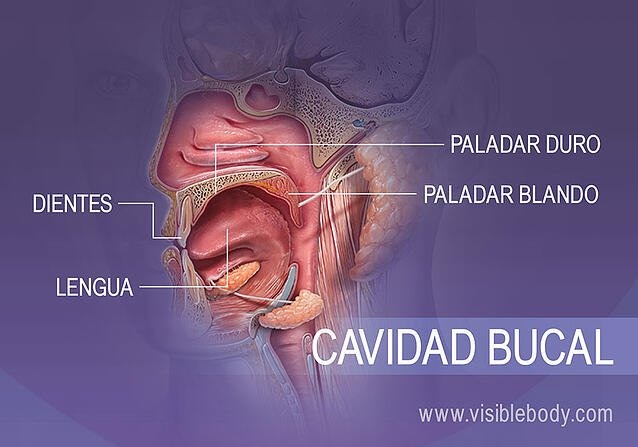
\includegraphics[width=0.8\textwidth]{cavidad_oral}
				\caption{Cavidad bucal}
				\label{fig:cavidad_oral}
			\end{figure}
		
			\subsubsection*{Componentes}
			
				\begin{itemize}
					\item Delimitada por \textbf{labios}, \textbf{mejillas}, \textbf{paladar} y \textbf{base de la boca}.
					\item Recubierta interiormente por la \textbf{mucosa bucal}.
					\item \textbf{Lengua}
					\item \textbf{Dientes}
					\item 3 pares de \textbf{glándulas salivales}.
					\item 2 \textbf{amígdalas}.
				\end{itemize}
				
			\subsubsection*{Los dientes}
			
				En total, hay 32 dientes. En cada maxilar:
				\begin{itemize}
					\item 4 incisivos, para cortar.
					\item 2 caninos, para desgarrar.
					\item 4 premolares y 6 molares, para triturar.
				\end{itemize}
				
				\begin{figure}[htp]
					\centering
					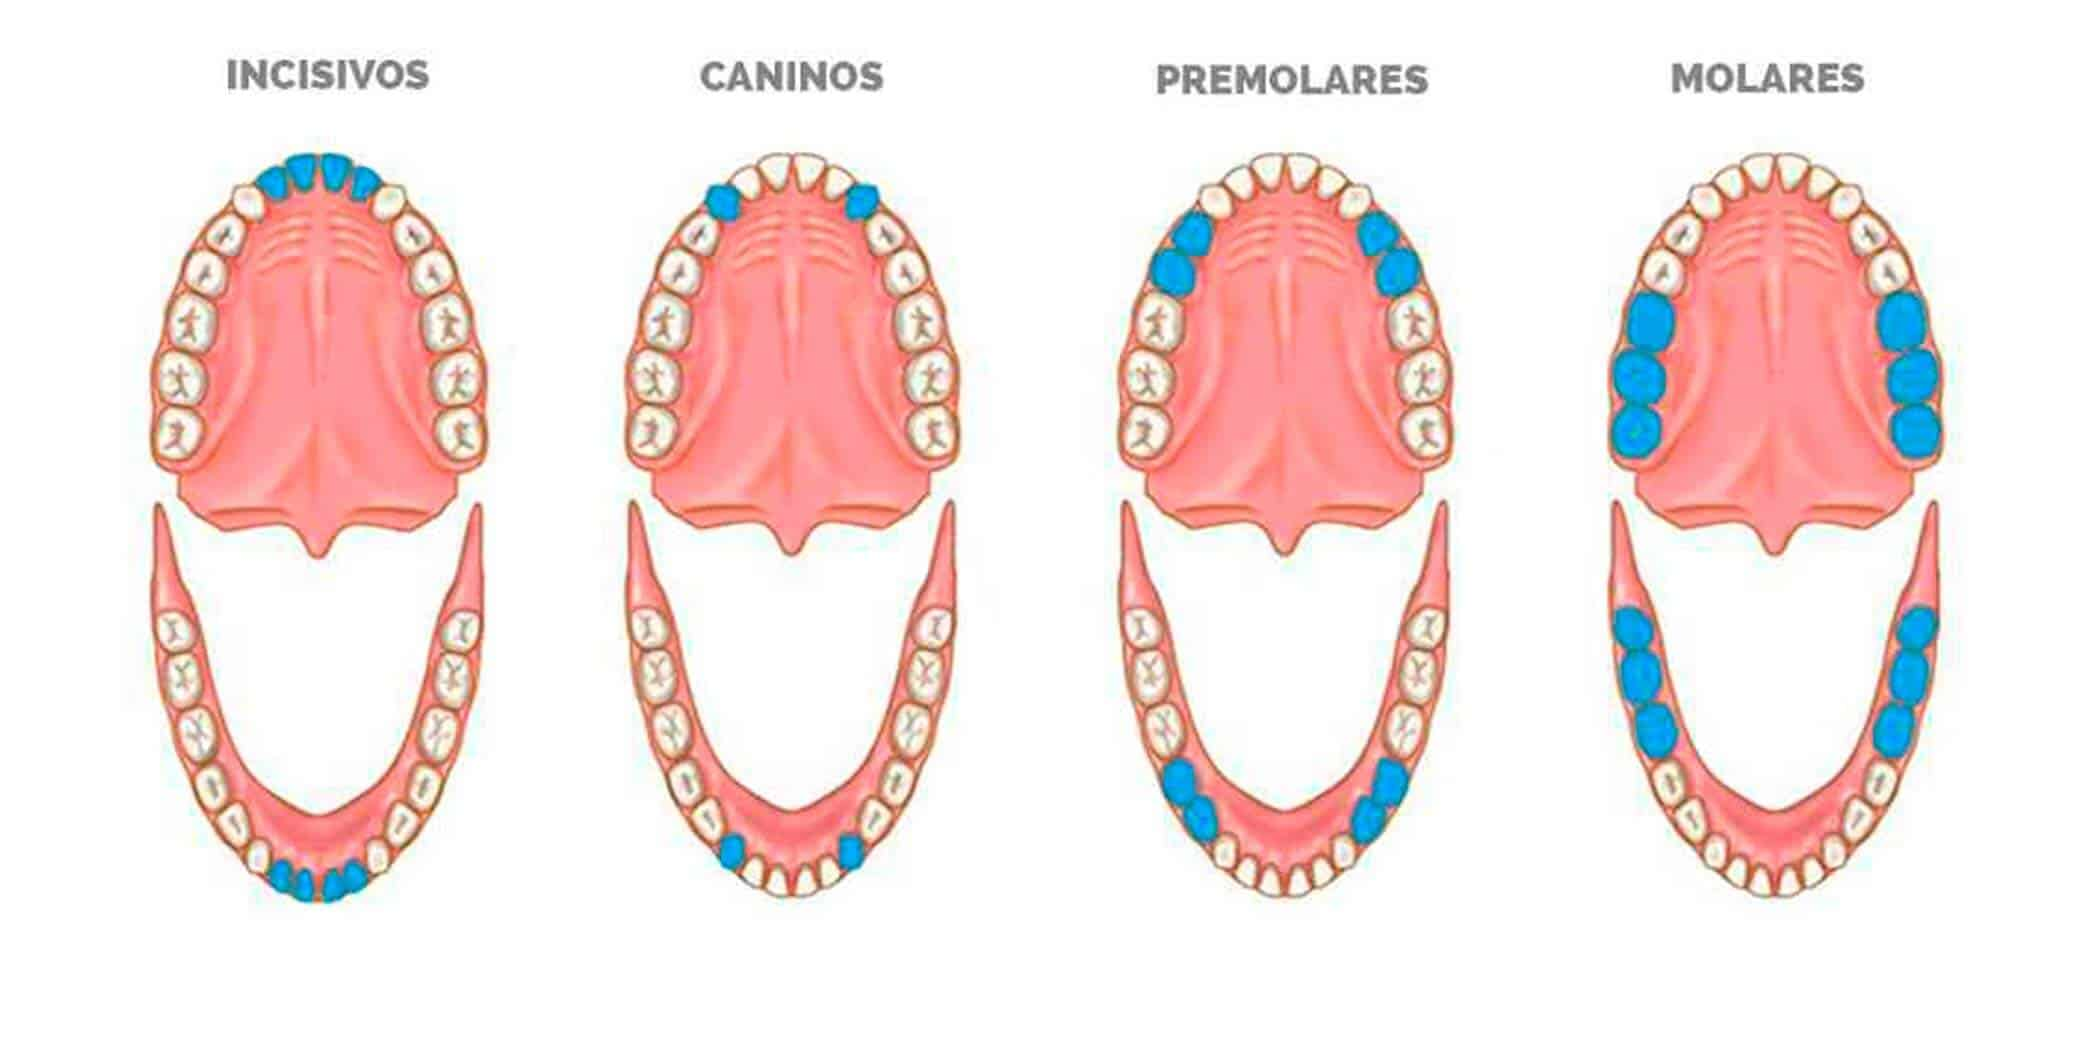
\includegraphics[width=0.8\textwidth]{dientes}
					\caption{Distribución de los dientes}
					\label{fig:dientes}
				\end{figure}
			
			\subsubsection*{Transtornos}
			
				La \textbf{caries dental} es la destrucción de los tejidos duros de los dientes y la inflamación de la pulpa dentaria, debido a la acción de unas bacterias.
				
		\subsection{El tubo digestivo hasta el estómago}
		
			\subsubsection*{La faringe}
				Se comunica con la laringe, con las fosas nasales y con el oído medio. Una lengüeta llamada \textbf{epiglotis} la separa de la laringe, impidiendo que el alimento penetre en la tráquea.
			
			\subsubsection*{El esófago}
			
			\subsubsection*{El estómago}
				Es un ensanchamiento con unos 2,5 L de capacidad. Las paredes presentan dos gruesas capas de músculo y están tapizadas de una mucosa, donde se encuentran las glándulas que secretan el \textbf{jugo gástrico}	
				
		\subsection{Las glándulas digestivas del estómago}
		
			\subsubsection*{El hígado}
			
				\begin{tabularx}{\textwidth}[htp] { 
  					| >{\centering\arraybackslash}X 
  					| >{\centering\arraybackslash}X 
  					| >{\centering\arraybackslash}X | }
 					\hline
 					\textbf{Función glandular} & \textbf{Función metabólica}  & \textbf{Función hemática} \\
 					\hline
 					Produce la bilis, un líquido que participa en la digestión de las grasas, y que se almacena en la vesícula biliar & Almacena glucógeno, sintetiza proteínas y desintoxica  & Forma y recicla la sangre, acumula hierro y vitamina K  \\
					\hline
					
				\end{tabularx}		

			\subsubsection*{Transtornos del hígado}
			
				La \textbf{hepatitis} es una inflamación del hígado que provoca que no funcione bien. Puede tener un origen vírico o deberse al excesivo consumo de alcohol.
			
			\subsubsection*{El páncreas}
			
				\begin{tabularx}{\textwidth}[htp]{
				| >{\centering\arraybackslash}X
				| >{\centering\arraybackslash}X | }
				\hline
				\textbf{Función exocrina} & \textbf{Función endocrina} \\
				\hline
				Libera el \textbf{jugo pancreático}, que contiene muchas enzimas digestivas & Libera \textbf{hormonas} a la sangre, destacando la \textbf{insulina} y el \textbf{glucagón} \\
				\hline 
				\end{tabularx}
			
			\subsubsection*{Transtornos del páncreas}
			
				\begin{itemize}
					\item \textbf{Diabetes de tipo I}. Se debe a que el sistema inmunitario destruye las células que producen la insulina. No puede prevenirse.
					\item \textbf{Diabetes de tipo II}. El páncreas produce una cantidad insuficiente de insulina. Se suele asociar a una ingesta excesiva de azúcares.
				\end{itemize}
						
\end{document}